\documentclass[14pt]{extreport}
\usepackage[utf8]{inputenc}
\usepackage[T2A]{fontenc} 
\usepackage[russian]{babel}
\usepackage{graphicx}
\usepackage{amsmath, amssymb}
\usepackage{geometry}
\usepackage{indentfirst}
\usepackage{hyperref}
\usepackage{fancyhdr}
\usepackage{afterpage}

\geometry{a4paper, left=30mm, right=10mm, top=20mm, bottom=20mm}

\setlength{\parindent}{1.25cm}
\setlength{\parskip}{0pt}

\linespread{1.5}

\pagestyle{fancy}
\fancyhf{}
\cfoot{\thepage}
\renewcommand{\headrulewidth}{0pt}

\begin{document}

\begin{titlepage}
\centering
\vspace*{2cm}
{\Huge \textbf{Реферат на тему:}} \\[1cm]
{\huge \textbf{Влияние искусственного интеллекта на современное образование}} \\[3cm]
{\Large Студент: Степанова Анна Андреевна} \\
{\Large Группа: ИВТ-1.2} \\[1cm]

\end{titlepage}

\cfoot{}

\tableofcontents
\newpage

\cfoot{\thepage}

\chapter{Введение}
Искусственный интеллект (ИИ) активно внедряется в различные сферы жизни. В образовании он открывает новые возможности для персонализации обучения, автоматизации проверки заданий и создания адаптивных курсов.

\chapter{Основная часть}
\section{Что такое ИИ в образовании}
ИИ в образовании — это использование алгоритмов машинного обучения и нейросетей для улучшения процессов преподавания и усвоения знаний.

\subsection{Примеры применения}
\begin{itemize}
\item Автоматическая проверка эссе
\item Персонализированные траектории обучения
\item Чат-боты-тьюторы
\end{itemize}

\subsection{Преимущества и риски}
\textbf{Преимущества:} доступность, скорость, адаптивность. \\
\textit{Риски:} потеря человеческого контакта, предвзятость алгоритмов.

\section{Статистика использования}
Ниже представлена таблица с данными по внедрению ИИ в вузах России.

\begin{table}[h]
\centering
\begin{tabular}{|c|c|c|}
\hline
Год & Доля вузов с ИИ-системами & Рост, \% \\
\hline
2020 & 12\% & -- \\
2022 & 28\% & +16\% \\
2024 & 45\% & +17\% \\
\hline
\end{tabular}
\caption{Внедрение ИИ в российских вузах}
\label{tab:ai}
\end{table}

\section{Иллюстрация}
На рисунке \ref{fig:ai} показана схема взаимодействия студента и ИИ-помощника.

\begin{figure}[h]
\centering
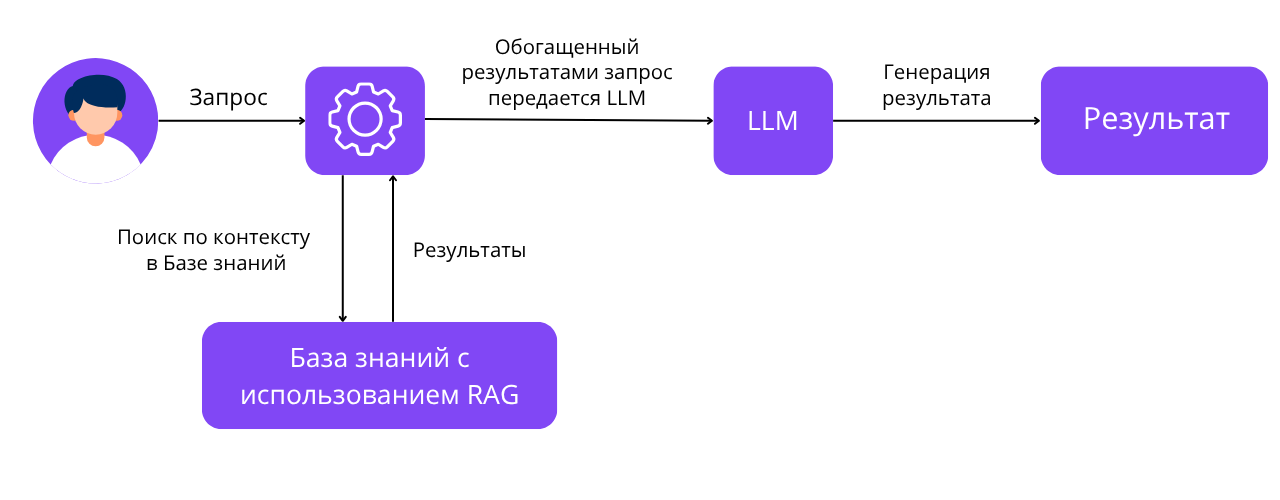
\includegraphics[width=0.5\textwidth]{image.png}
\caption{Схема ИИ-тьютора}
\label{fig:ai}
\end{figure}

\chapter{Заключение}
ИИ становится неотъемлемой частью образования. Его грамотное использование повышает качество обучения, но требует внимания к этическим вопросам.

\section*{Список литературы}
\begin{enumerate}
\item Татьяна, В. Б. Искусственный интеллект в образовании: современное состояние и перспективы развития / В. Б. Татьяна. — Текст : электронный // CyberLeninka : [сайт]. — URL: \url{https://cyberleninka.ru/article/n/iskusstvennyy-intellekt-v-obrazovanii-sovremennoe-sostoyanie-i-perspektivy-razvitiya} 
\item Аманова, Ай Влияние искусственного интеллекта на современное образование / Ай Аманова. — Текст : электронный // CyberLeninka : [сайт]. — URL: \url{https://cyberleninka.ru/article/n/vliyanie-iskusstvennogo-intellekta-na-sovremennoe-obrazovanie}
\item Майорова, П. Д. Искусственный интеллект в образовании: трансформация процессов обучения и новые вызовы / П. Д. Майорова. — Текст : электронный // moluch.ru : [сайт]. — URL: \url{ https://moluch.ru/archive/594/129400}
\end{enumerate}

\end{document}
